\chapter{Introduction}\label{chp:introduction}

The web is becoming the primary platform for all communication, as people gradually move away from the solutions provided by their telco operator, such as telephony and text messaging. Moving audio conversations to the Internet has been relatively easy, but as we're now commoditizing video conversations, moving away from custom rooms and dedicated hardware over the regular laptops and phones, the most straightforward solutions lead to performance requirements greater than most user equipment and their connections can handle.

There are lots of competing products on the market today, with different characteristics and performance levels. What they all have in common however, is that they've all chosen a fixed network topology, which dictates most of their expected performance. The goal of this thesis is to investigate the feasibility of designing a system which does not have a fixed topology, but choses one adaptively based upon properties of the user equipment and connection quality in a given conversation.

\todo[inline]{Write about what WebRTC is how that changes the playing field for real-time communication}

The goal of this project is to maximize user utility in video conference solutions. To maximize utility, we need to have a well-defined sense of what that implies.


\section{Context and utility}

When defining user utility, context is everything. You have different expectations to audiovisual quality on a desktop computer with fiber connectivity compared to your phone on 3G. But how can this difference be quantized? Certainly it's not a question of screen resolution, as most smart phones today have the same 1080p resolution as most computer screens. Resolutions beyond 1080p, like we can find on some "retina" screens, are not that interesting for video conferencing, as the webcam producing the source video is unlikely to be able to keep pace.

However, physical screen size matters. Viewing distance matters. Latency matters very much. Bandwidth matters. Packet loss matters. Most of these should be fairly easy to estimate, but then we have a new problem: which of these attributes do we prioritize? Finding the optimal balance is the key to optimizing user utility. There are of course also non-technical factors that affects the expected experience quite much that cannot be determined by the device itself. For example, even though the device is the same, you'll have different expectations sitting on the bus to work compared to sitting in a sofa in your living room, even though the device and maybe even the connection is the same. Content matters. Environment matters. Mood matters. Time of day probably matters. We will however not take all of these factors into account, but limit our scope to the device and the connection, and since the intended application is to WebRTC, what we can relatively easy determine through the browser.

There will also be diminishing returns on most of these metrics. If you have practically unlimited bandwidth available, there's little to gain from sending video with bitrates in excess of 3 Mbps, you'll just be wasting bandwidth, CPU and battery. If we define a quality threshold for a device as the "optimal" experience that can be attained as 1.0, there's no reason to try to push this as high as possible. We can though assume that all metrics that are lower than what's necessary for this optimal experience will subtract from this quality metric somehow. For example, if we say that the threshold for optimal latency for a device is \(20ms\), we can imagine a \gls{utility function} that behaves like \(1 - x^t\), where t is a constant determining how fast this metric deteriorates. The general function is illustrated in \autoref{fig:utility-latency}.

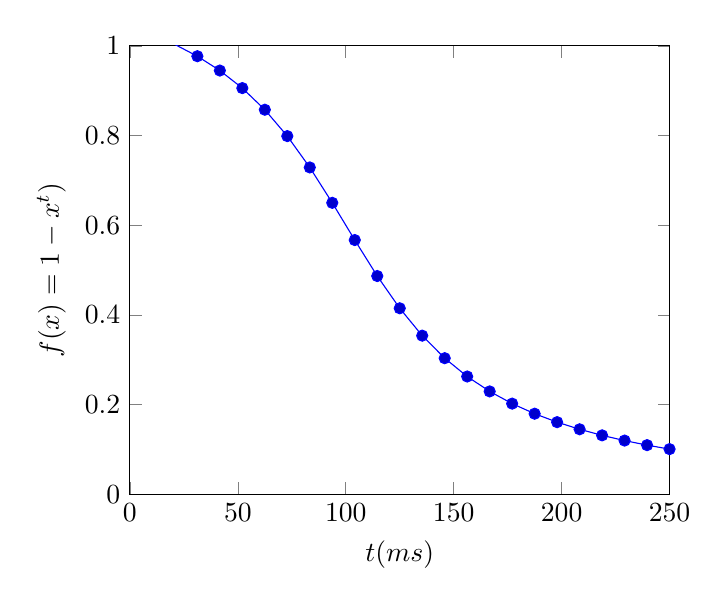
\begin{tikzpicture}
    \begin{axis}[
        xlabel={$t (ms)$},
        ylabel={$f(x) = 1 - x^t)$},
        xmin=0,
        ymin=0,
        ymax=1,
        xmax=250]

    \addplot+[domain=0:250]{0.6 + 0.4*rad(atan(20*0.1 - 0.02*x))};
    \label{fig:utility-latency}
    \end{axis}
\end{tikzpicture}

For now we'll assume that we have a function similar to the one illustrated in \autoref{fig:utility-latency}, returning a value approximately in the range \todo{Find the proper lower limit}\(1 -- 0\), for each of the metrics that comprise the user utility. Multiplying these together we'll get a user utility that lies in the same range.

Assuming this user utility function, we have to figure out what to optimize in a conversation. If a single party in a conversation experiences high latencies and much packet loss, it's likely to negatively affect the experience of all the other parties as well, due to that person requesting people to repeat what they said and being hard to hear for other participants. We'll thus focus on maximizing the minimum utility experienced in a conversation, and then gradually improve the utility for all users ordered by their current utility in ascending order.

To narrow down the problem scope a little, let's define some example conversations to work it, and assume that if we can efficiently serve these setups, we can serve most others as well. The conversations we'll use are given in \autoref{tab:example-conversations}.

\todo{Maybe graph these on a map to illustrate the latencies between them and the servers?}
\begin{center}
    \label{tab:example-conversations}
    \begin{tabular}{| l | l |}
    \hline
    \textbf{Case} & \textbf{Devices} \\ \hline
    Casual & A (laptop, 20/5), B (laptop, 30/15) \\ \hline
    Casual & A (laptop, 10/2), B (laptop, 30/5), C(phone, 2/1) \\ \hline
    Business & A (desktop, 50/50), B (desktop) \\ \hline
    \end{tabular}
\end{center}

Are there any trivial cases we can ignore? As long as there's only two people in a conversation, and they have fairly low latency between each other and sufficient bandwidth, peer-to-peer is the optimal choice in all cases. Initially, it might seem like this would indeed be the case in all conversations with two participants, and not just the good bandwidth, small latency case. However, this is not the case. To illustrate why, consider a conversation between two people, one in Europe and one in Asia. The latency between them is ~350ms. They both have fairly acceptable bandwidths, with 3Mbps each, which should be plenty to sustain an acceptable video link between them. This, however, is not the case, as the bandwidth between them is far more limited due to the long distance and many hops through publicly routed networks. However, each of the peers has a datacenter of a distributed VPS provider nearby, to which they can utilize their full bandwidth. And these distributed VPS providers tend to have established high-quality routes between their own datacenters, SLA-backed and with all the bells and whistles you don't get on your private Internet connection. Thus, the available bandwidth between the two datacenters is far greater than what can be achieved directly between the two peers. Thus, their video link can be improved by routing their traffic through the datacenters, thus enabling each peer to utilize the full bandwidth of their connection.\footnote{This is backed by a simple experiment, using DigitalOcean as our VPS provider. From a 100Mbit university connection in Norway, sustained datarates to their Singapore datacenter varied greatly, measuring 90kBps, 3,7MBps, 1,9MBps and 2,58MBps for each test. However, from their Amsterdam datacenter, a consistent throughput of 24,6MBps was measured} Do however note that the latency is close to unchanged from routing through the datacenters, only sustained bandwidth between the peers is improved.

These conversations are not extensive, but should cover enough corner cases to be able to highlight the pros and cons of the different topologies. The examples cover the low-latency, few peers conversations; the bandwidth-challenged cases; the high-latency conversations; and the very hetrogenous device conversations, where one or more party is severly challenged in terms of either bandwidth or latency.

We assume that the backend networks are not saturated, and that each user is bandwidth-constrained only by their connection. By extension, the maximum bandwidth attainable between any pair of nodes in our network is the lesser of the upload bandwidth of the sending party and the download bandwidth of the receiving party. However, latency has to be defined for any pair of the nodes in the network, as this is mostly determined by their geographical location in relation to each other. To best illustrate the physical topology, we can draw each scenario as a complete graph:

\begin{figure}[ht!]
\centering
    \digraph{exampleconvchat}{
        edge [dir=none];
        rankdir=LR;
        a [label="A (20/5)"];
        b [label="B (30/15)"];

        a -> b [label="8ms"];
    }
    \caption{Example conversation "chat".}\label{fig:example-conv-chat}
\end{figure}

\begin{figure}[ht!]
\centering
    \digraph{exampleconvcasual}{
        edge [dir=none];
        rankdir=LR;
        a [label="A (10/2)"];
        b [label="B (30/5)"];
        c [label="C (2/1)"];

        a -> b [label="5ms"];
        a -> c [label="10ms"];
        b -> c [label="15ms"];
    }
    \caption{Example conversation ``casual''}\label{fig:example-conv-casual}
\end{figure}

\begin{figure}[ht!]
\centering
    \digraph{exampleconvbusiness}{
        edge [dir=none];
        a [label="A (50/50)"];
        b [label="B (50/50)"];
        c [label="C (50/50)"];
        d [label="D (30/30)"];
        e [label="E (30/30)"];

        a -> b [label="2ms"];
        a -> c [label="2ms"];
        a -> d [label="150ms"];
        a -> e [label="150ms"];
        b -> c [label="2ms"];
        b -> d [label="150ms"];
        b -> e [label="150ms"];
        c -> d [label="150ms"];
        c -> e [label="150ms"];
        d -> e [label="2ms"];

        {rank=same; a; c;}
        {rank=same; d; e;}
    }
    \caption{Example conversation ``business''}\label{fig:example-conv-business}
\end{figure}


\section{Previous and Related Work}

\epigraph{If I have seen further, it is by standing on the shoulders of giants}{Isaac Newton}

Networking and algorithms related to networking is not a new topic, by any stretch of the imagination, and like in all most branches of computer science, it's mostly old problems in a new context.

During this thesis we will borrow heavily from previous work on networking and graph algorithms in general, and flow algorithms in particular. Many algorithmic problems can be solved as a linear program, which as a problem was first solved by Fourier in 1827\cite{sierksma2001linear}. Another solution, the simplex method, was first introduced by G.B. Dantzig in 1947\cite{sierksma2001linear}, and was first introduced to me in \cite{ahuja1988network} by Ahuja, Magnanti and Orlin, and serves as the basis for much of our suggested solution. The simplex method has been widely adopted for its ease of implementation on computers, and years of exponential growth of computer performance has made increasingly large problem sets solvable in realistic time.

Now that we've established the problem domain and have some grasp of the main challenges, let's see where we are today.


\section{Disclaimer}

This thesis does not try to measure or optimize for audio transmission, as that's a much simpler problem that can practically always be completed by sending the same stream to all nodes in the conversation. There's always only one stream to encode, it doesn't noticably affect available bandwidth, and it's already widely deployed. However, results we achieve for video can also be applied to audio streams if the environment is very heavily constrained or further optimization is required, it's just not the focus of this thesis.
